
% Background and Significance
% No page limit
\chapter{Background: Neuroimaging for the Examination of Anatomy, Structure and Function in the Human Brain }
\label{chap_back}

The modern development of methods for in-vivo imaging of the human brain is indispensable for understanding of brain function and malfunction. While techniques such as positron emission tomography (PET) provide the ability to image brain activation, the significantly better spatio-temporal resolution provided by magnetic resonance imaging (MRI) has made it the technique of choice for identifying anatomy and in studies of both structure and function in the brain. Different tissue types are distinguished by MRI based upon the levels of hydrogen that they contain. Because white matter contains a large amount of tissue, while gray matter has many fluid-containing cell bodies, MRI is particularly good for distinguishing between these tissue types. The versatility of MRI has led to the development of techniques to measure structure and function in the brain, providing a framework for examining the relationship between structural and functional connectivity and their role in modulating behavior.

% DTI
\section{Diffusion Tensor MRI}
Of particular interest in this dissertation is the use of diffusion tensor MRI in the examination of structural and anatomical connectivity. Diffusion tensor imaging provides an in-vivo non-invasive measure of the local probability of self-motion of water molecules and has proven useful in a number of applications for the study of brain white matter~\cite{Basser1994}. The diffusion of water in white matter is highly anisotropic due to cell walls and myelin which inhibit diffusion perpendicular to the fiber tracts more so than diffusion parallel to the tracts. Both the shape and orientation of the diffusion tensor provide important information regarding the structure of the white matter. Scalar metrics derived from the diffusion tensor, such as fractional anisotropy (FA) and mean diffusion (MD) are often used to quantify various tissue properties. The structural information provided by the diffusion tensor has been shown to be useful in a multitude of studies examining topics such as neurodegenerative disorders, traumatic brain injury, development, and aging among others~\cite{Lebel2008,Sydykova2007,Xu2007}.

\subsection{Diffusion weighted MRI}
% Molecular Diffusion
The constant random motion of particles in liquids, known as Brownian motion, provides a method for using MRI to measure the self-diffusion of water.  As the particles move they collide with other particles and over time the path of any given particle may be described by a random walk.  In the presence of a concentration gradient, a flux of the fluid is observed.  If no concentration gradient is present it becomes necessary to describe diffusion as the statistical probability that a particle moved a certain distance in a given time.  Einstein~\cite{Einstein} showed that such a probability has a zero-mean Gaussian distribution with a variance that is proportional to time:
$$ <r^2> = 2NDt, $$
where $D$ is the diffusion coefficient, $t$ is time, and $N$ is the number of spatial dimension over which distances are measured.

% Measuring Diffusion with MRI
In the case of MRI, diffusion may only be measured in one direction at a time, so $N$ is equal to one.  As spins in the presence of a magnetic field gradient diffuse, they accumulate phase shifts, thus reducing the intensity of the MR signal.  This effect may be magnified with the use of stronger gradients, and may be accurately measured with a spin-echo sequence such as the one illustrated in Figure~\ref{fig:sequence} that includes equal rectangular gradient pulses both before and after the refocusing pulse.  During the first pulse, spins acquire different phase shifts based upon their location.  If the spins remain stationary, then these phase shifts are reversed during the second pulse.  Spins that diffuse however will acquire a net phase shift resulting in a signal attenuation, $A$, that is proportional to the diffusion coefficient, $D$, according to
\begin{equation}
\label{eq:attenuation1}
A = e^{-bD}
\end{equation}
where $b$ is the 'b-factor', a quantity characterized by the amplitude, shape, and timing of the magnetic field gradient used for acquisition.

\begin{figure}[ht]
\begin{center}
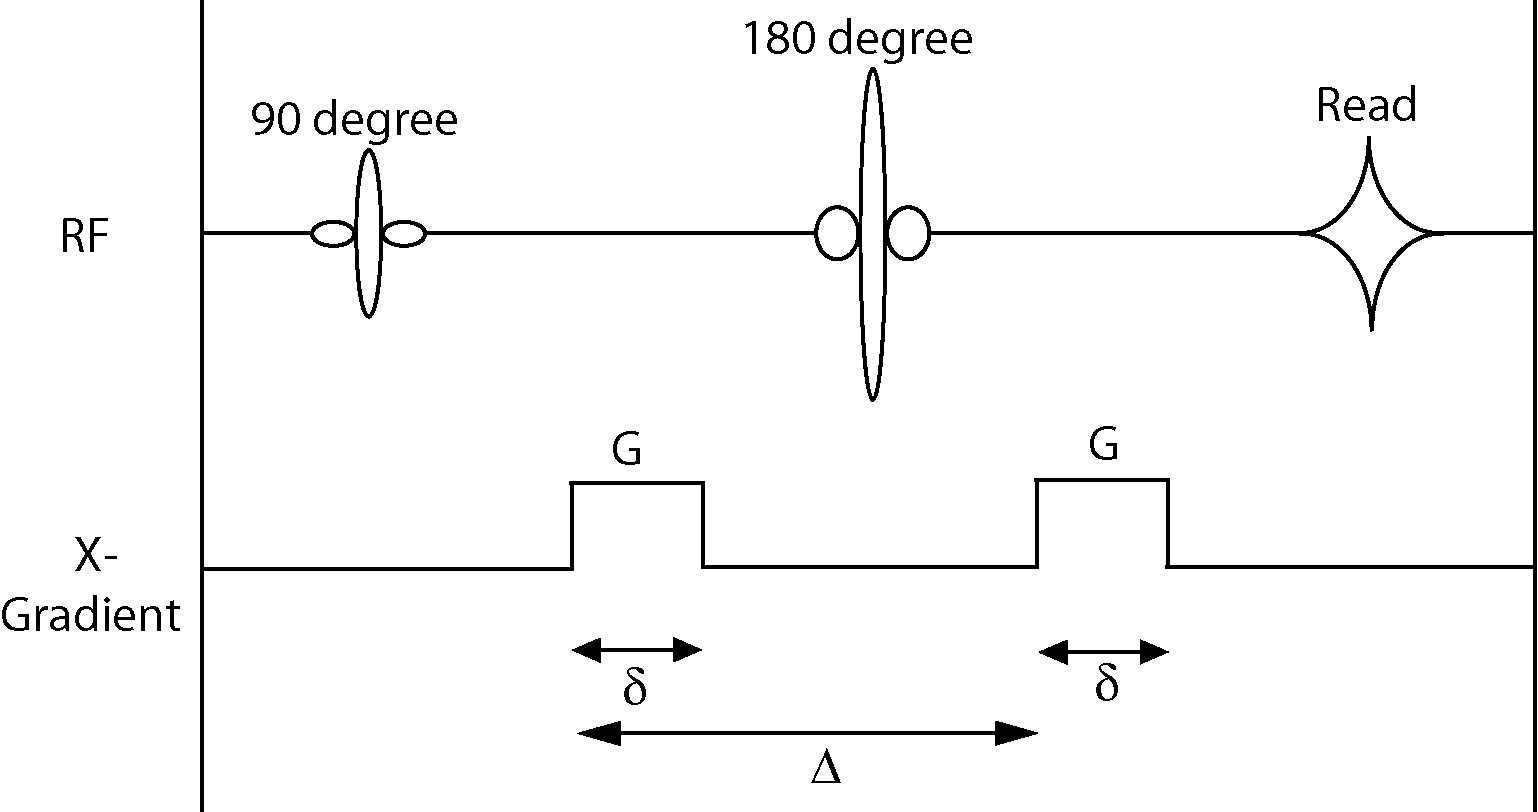
\includegraphics[width=4in]{figures/sequence}
\caption{
\label{fig:sequence}
An example diagram of a Stejskal-Tanner pulse gradient spin echo experiment used to measure diffusion (adapted from ~\cite{Behrens2004}).  For further explanation on understanding pulse sequence diagrams, please see \cite{Haacke}.}
\end{center}
\end{figure}

% Measuring the Tensor
\subsection{Measuring the diffusion tensor}
In the case of isotropic tissue, diffusion may be described by a single scalar parameter, the diffusion coefficient.  However, tissue such as white matter is anisotropic and in order to fully characterize the diffusion it is necessary to use a tensor which describes diffusion along each direction and the correlations between these directions \cite{LeBihanJMRI2001}.  Mathematically, a symmetric, second order tensor, $D$, is used to describe the three dimensional self-diffusion of water within a volume:
$$ \underline{D} = \begin{pmatrix} 
	D_{xx} & D_{xy} & D_{xz} \\
	D_{yx} & D_{yy} & D_{yz} \\
	D_{zx} & D_{zy} & D_{zz}
	\end{pmatrix}
$$
The principle directions of diffusivity may be used to define a reference frame [$x', y', z'$] .  In this case, the diagonal terms of the tensor, $D_{x'x'}, D_{y'y'}, D_{z'z'}$, may be used to represent diffusion along [$x', y', z'$] and the attenuation becomes
\begin{equation}
\label{eq:attenuation3}
A = e^{-b_{x'x'}D_{x'x'} - b_{y'y'}D_{y'y'} - b_{z'z'}D_{z'z'}}
\end{equation}
where $b_{ii}$ are elements of the b matrix which expresses the b-factors for the directions in the reference frame.  However, measurements are actually made in a frame of reference [$x,y,z$] defined by the scanner.  This makes it necessary to incorporate the non-diagonal elements of the \underline{b} matrix in order to incorporate the correlation of diffusion in perpendicular directions, leading to
\begin{equation}
\label{eq:attenuation6}
A = e^{- \sum_{i=x,y,z}{ \sum_{i=x,y,z}{ \underline{b}_{ij}\underline{D}_{ij} } } }
\end{equation}
Because the diffusion tensor is symmetric, $D_{ij} = D_{ji}$, the attenuation may also be written as
\begin{equation}
\label{eq:attenuationfull}
A = e^{-b_{xx}D_{xx} - b_{yy}D_{yy} - b_{zz}D_{zz} - 2b_{xy}D_{xy} - 2b_{xz}D_{xz} - 2b_{yz}D_{yz} }
\end{equation}
In order to determine the diffusion tensor it is necessary to obtain six or more measures of attentuation, which requires a minimum of six diffusion weighted images and one non-diffusion weighted image.
  
The eigensystem of $D$ consists of three eigenvectors, $e_1, e_2, e_3$ and their corresponding eigenvalues $\lambda_1  \le \lambda_2 \le \lambda_3$. The eigenvectors describe the principal axes of diffusion, and the eigenvalues are proportional to the mean squared displacements along the corresponding eigenvector. The values may be used to define visualization of tensor such as ellipsoids with orientation determined by eigenvectors and size determined by eigenvalues. The mapping of the components of $e_1$ into an RGB-color space is known as a directionally encoded color (DEC) map~\cite{Pajevic1999}.
  
\begin{figure}[ht]
\begin{center}
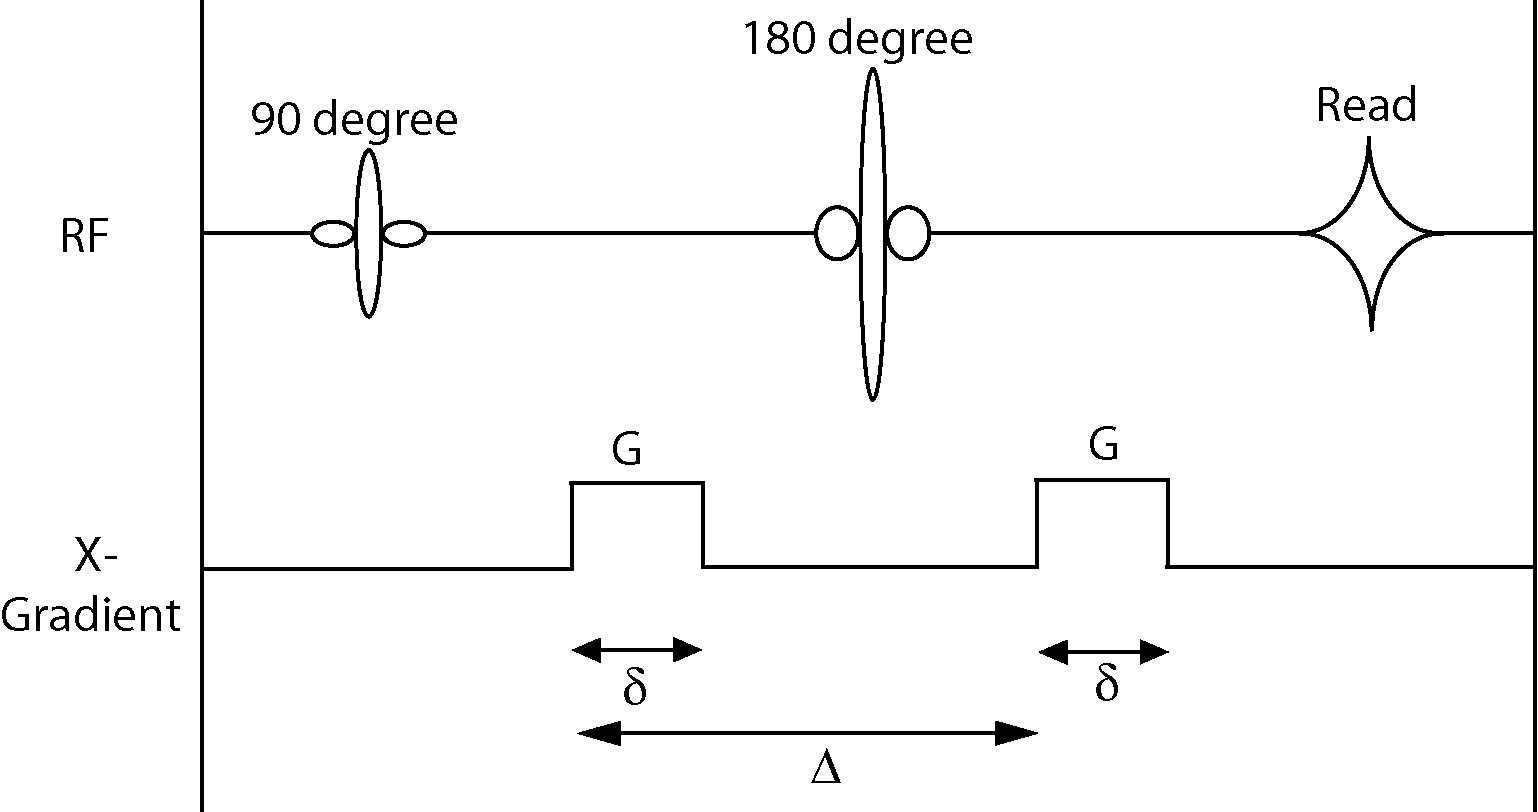
\includegraphics[width=4in]{figures/sequence}
\caption{
\label{fig:sequence}
An example diagram of a Stejskal-Tanner pulse gradient spin echo experiment used to measure diffusion (adapted from Behrens thesis).  For further explanation on understanding pulse sequence diagrams, please see \cite{Haacke}.}
\end{center}
\end{figure}
  
% Diffusion in fibrous tisssue
In tissue, the diffusion of water may be anisotropic, i.e. it may vary with direction, due to the presence of obstacles that limit molecular movement.  The axons of white matter are insulated with a fatty protein called myelin which insulates the the axon improves the efficiency of signals that travel along the axon~\ref{fig:neuron}. In fibrous tissue such as white matter the arrangement of nerve fibers into bundles results in a bias in which diffusion parallel to the fibers is often 3-6 times faster than diffusion perpendicular to the fiber bundle \cite{LeBihanNATURE2003} due to the restriction of water diffusion caused by myelin and the cell walls of the axons.  This ability to estimate fiber bundle orientation within a voxel led to the field of fiber tractography.  

\begin{figure}[ht]
\begin{center}
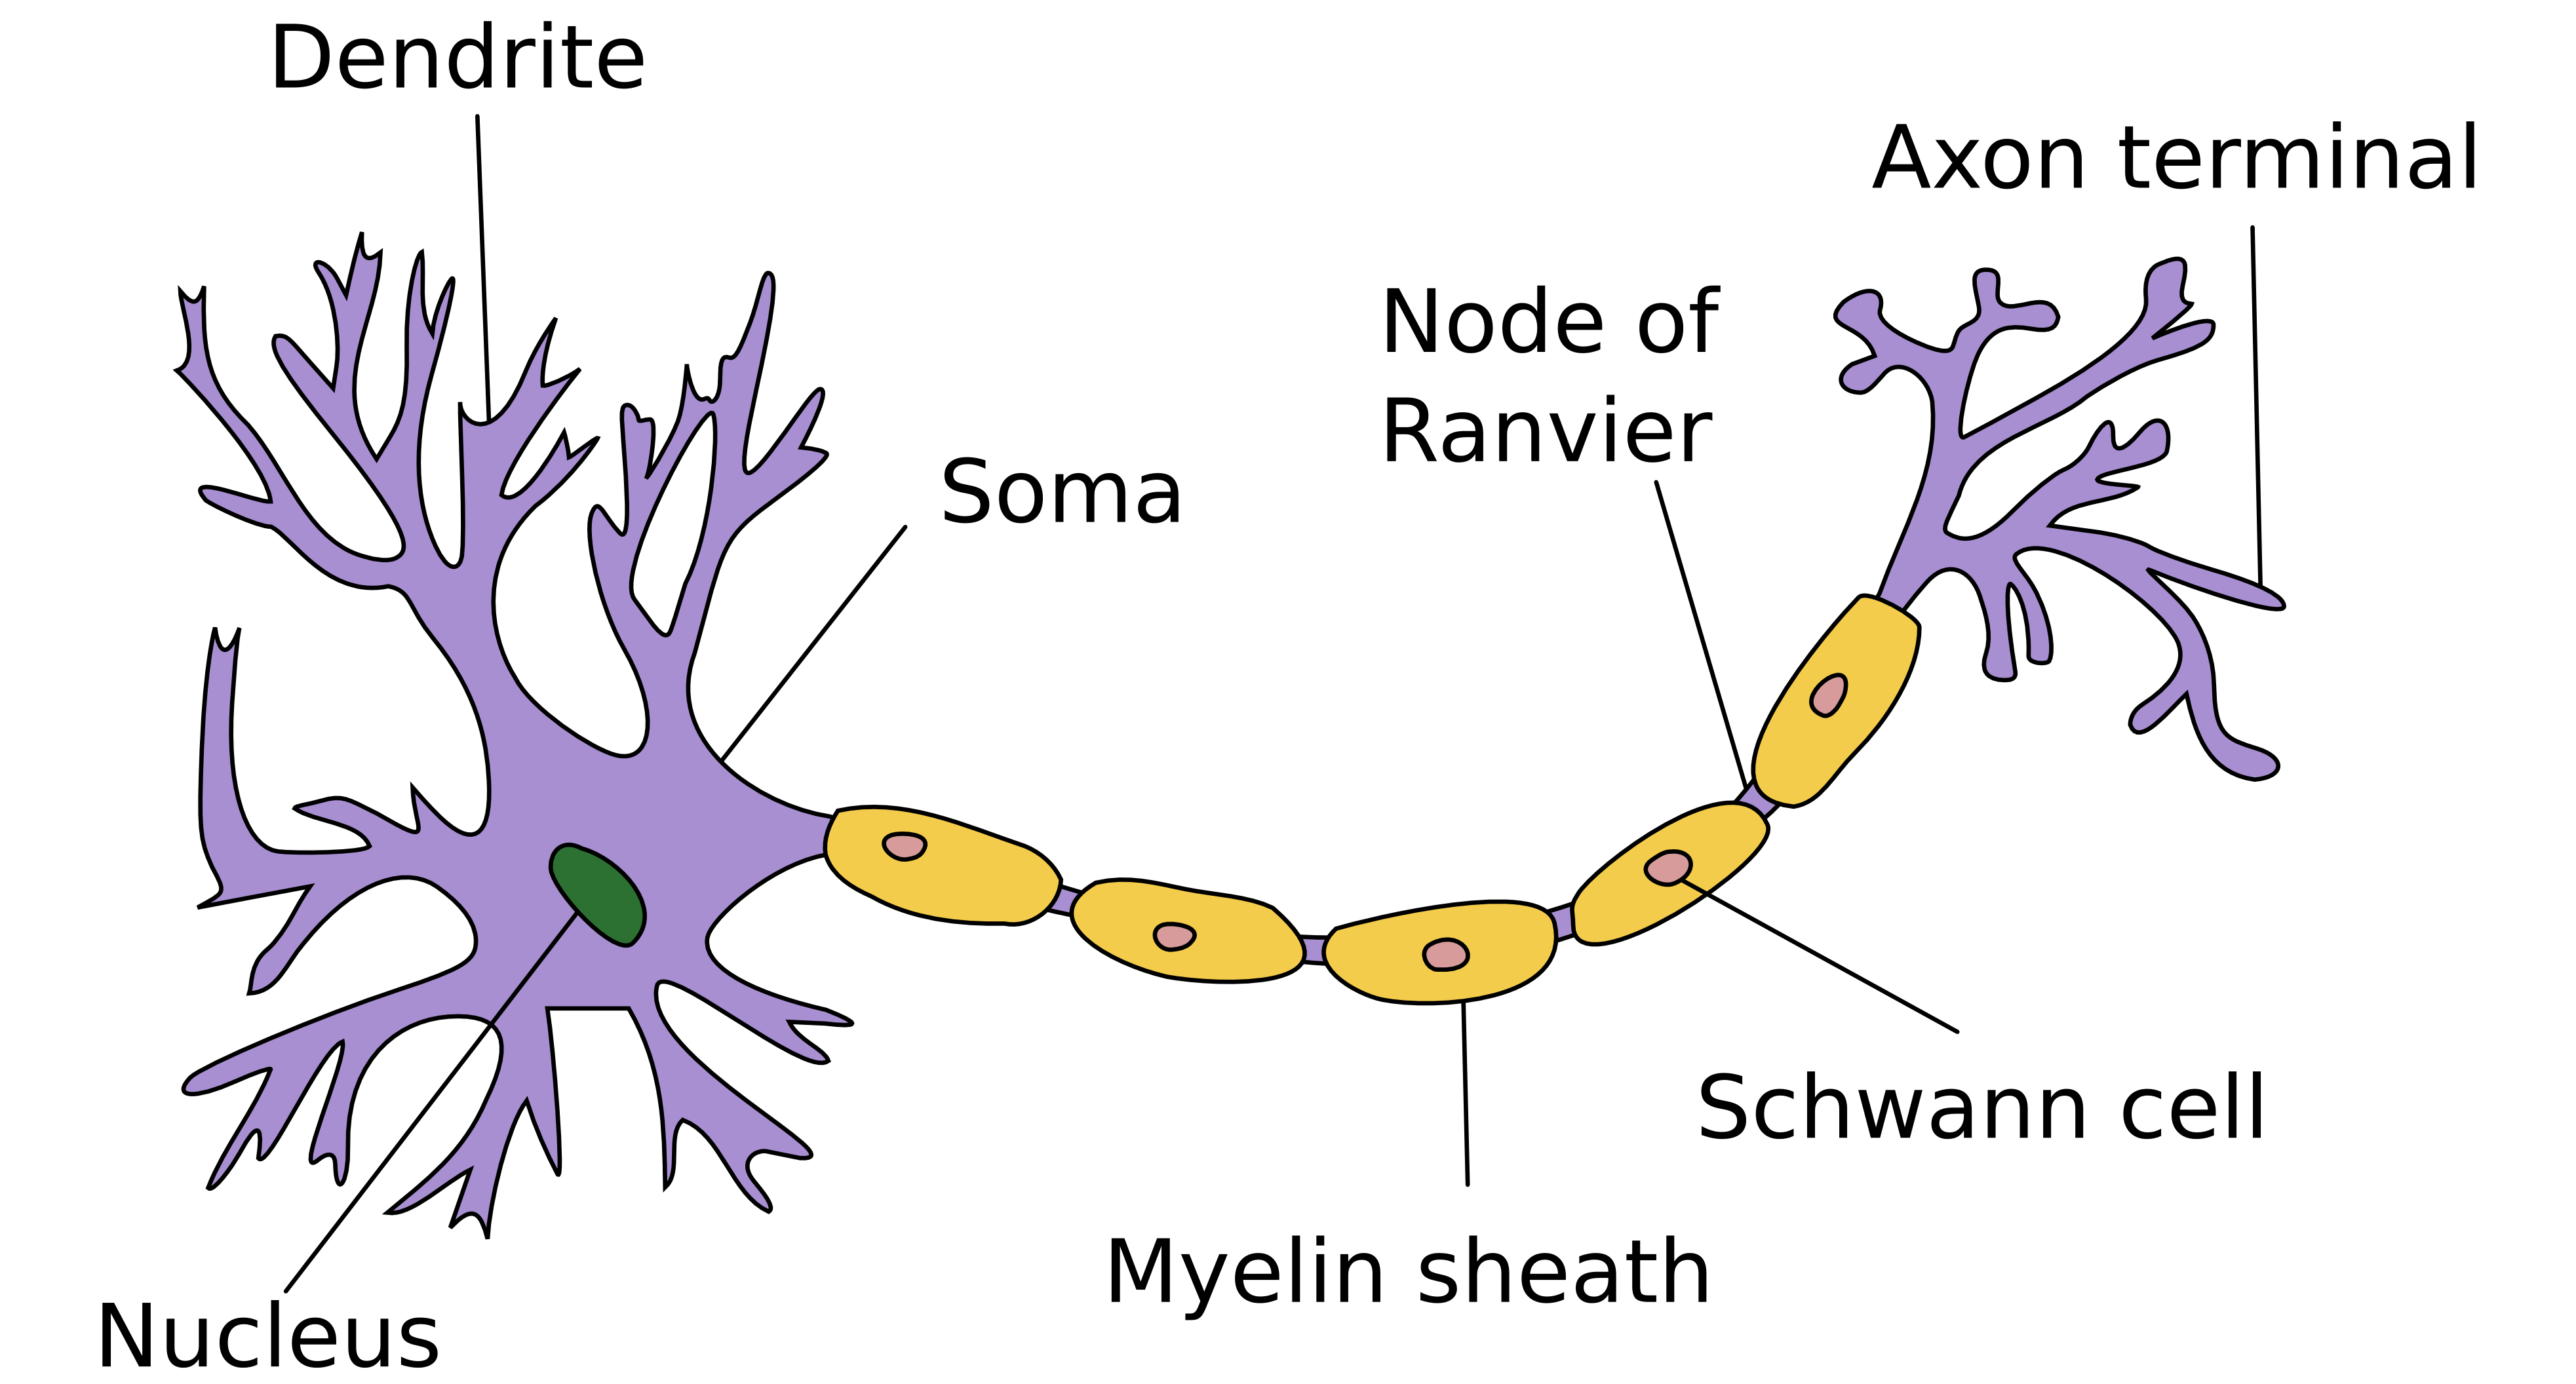
\includegraphics[width=0.75\linewidth]{figures/Neuron_Hand-tuned.png}
\caption{
\label{fig:neuron}
Diagram on a neuron with a myelinated axon (adapted from wikipedia).}
\end{center}
\end{figure}

\subsection{Fiber tractography}
A great deal of research focused upon methods for fiber tractography which use the fiber orientation information provided by the diffusion tensor to estimate trajectories of white matter fiber bundles throughout the brain. Tractography may provide a framework for identifying anatomical connections and studying the structural properties of the underlying white matter. Tractography methods can be grouped into 3 categories: deterministic, probabilistic, and energy-minimizing. 

\subsubsection{Deterministic tractography}
Deterministic tractography methods use a starting seed point, and then the direction information provided by the diffusion tensor is used to trace fiber trajectories until the end of a fiber bundle is reached~\cite{Basser2000,Mori99b}. These trajectories are referred to as streamlines. Due to the limited spatial resolution of DTI, streamlines represent estimated pathways of large bundles of fibers and do not correspond to the trajectories of individual axons. Methods for deterministic tractography typically differ in the details of the methods used to infer fiber direction from the underlying tensor field. Approaches include following $e_1$ from voxel to voxel~\cite{Mori1999}, linear interpolation of $e_1$ combined with a fixed step-size~\cite{Conturo1999}, linear interpolation with adaptive step-size using the Runge-Kutta method~\cite{Basser2000,Tench2002}, and methods that incorporate a momentum term to account to account for previous steps~\cite{Lazar2003}. To determine when then end of a fiber bundle has been reached, various stopping conditions are used such as FA thresholds~\cite{Conturo1999}, local curvature thresholds~\cite{Basser2000}, and measures of local orientation dispersion~\cite{Mori1999}

All deterministic methods suffer from error propagation resulting from noise in the DTI signal~\cite{Basser2000}. The extent of the error varies with the geometry of the fiber bundle, the anisotropy in the white matter, the resolution of the data, and the interpolation method~\cite{Lori1999}. Deterministic method may fail when a single voxel contains fibers from two or more distinct populations including fiber that cross, ``kiss", branch or merge~\cite{Basser2000}. One approach to avoid false-negative connections is a brute-force approach to seed selection known as whole-brain tractography. In this approach, all points in the brain are used as seeds for fiber tractography~\cite{Conturo1999}.
A lack of confidence measures for streamlines makes the automatic identification of spurious streamlines difficult. The use of user defined landmarks may reduce this problem but is time intensive and requires exiting knowledge of anatomy~\cite{Mori2002a,Wakana2004,Wakana2007}.

\subsubsection{Probabilistic tractography}
Probabilistic tractography methods use the fiber orientation measurements provided by diffusion weighted MRI to estimate the likelihood of a connection between two points. This likelihood is the integral of all possible paths that connect two points and is solved analytically by generating a set of ``probabilistic streamlines". At each point in the image, a local probability density function (PDF) of orientation is defined. A probabilistic streamline is traced by drawing a sample orientation from the PDF at each point and advancing by a small step along that direction. As with deterministic tractography, this advancement continues until a stopping criteria determines that the end of the fiber bundle has been reached. A final measure connectivity between two points is then determined by calculating the probabilistic index of connectivity (PICo), a quantity that was introduced independently by Parker et al.\ \cite{Parker2002} and Lazar and Alexander~\cite{Lazar2003}. Approaches to probabilistic tractography differ in the approach to estimating the PDF which include model-based approaches~\cite{Parker2002,Lazar2003} and a Bayesian approach~\cite{Behrens2004}. 

Model-based approaches to estimating the PDF are limited by the sources of uncertainty that may be included in the model. Uncertainty resulting from patient motion and eddy-current distortion are not included in the estimates of uncertainty. Additionally, these methods assume a Gaussian diffusion of water which is not necessarily the case. Probabilistic tractography methods are also sensitive to seed selection. Because a large number of streamlines are calculated for each seed (typically near 10,000) the whole-brain approach used in deterministic tractography may not be a practical option for examining human data. 

\subsubsection{Energy-minimizing tractography}
Energy-minimizing tractography approaches may be grouped into two categories, fast-marching and simulated annealing. Fast-marching methods rely upon level-set theory and the fast-marching algorithm. From a given seed point, the speed and direction of a propagation front are defined from local tensor properties. The use of local properties means that the propagation of the front will vary in different regions of the brain. Time-of-arrival maps are then determined for the whole brain and used to estimate the likelihood of a connections between a seed and any given point in the brain. These methods differ in the details of how the tensor data is used to define a speed and direction of the propagation front. Parker et al.\ \cite{Parker2002a} relied upon $e_1$ while O'Donnell et al.\ \cite{ODonnell2002} incorporated the whole diffusion-tensor. The simulated annealing approach considers two points, and attempts to identify the most favorable path that connects these points. Local energies at points along a potential path are determined based upon geometric properties of the path (short, straighter paths are generally preferred) and upon agreement between the direction of the path and the orientation of the underlying tensor field. Energy-minimizing methods differ in the details of how a local energy is determined~\cite{Tuch2000,Tuch2001}. Energy-minimizing approaches rely upon a priori knowledge of anatomy as they require the selection of two end points to examine. False-positive connections are also a problem as these methods are guaranteed to fine some level of connectivity between any two points, even when that connection is not anatomically feasible. While these methods present potential solutions to the problems caused by fiber crossing and branching, little has been done to evaluate the methods or demonstrate their performance in clinical data.

%fMRI
\section{Functional MRI}
Brain activation may be mapped with MRI by exploiting the interrelationship between physiological function, energy metabolism and localized blood supply. In particular, the blood-oxygenation-level-dependent (BOLD) contrast mechanism first demonstrated by Ogawa, et al.~\cite{Ogawa1990}, has been employed extensively due to its high sensitivity and accessibility. The BOLD contrast results from gradient echo techniques that accentuate the susceptibility effects of deoxyhemoglobin (dHb) in the venous blood and thus reflects the blood oxygen level. While increased neural activity should result in a decreased BOLD signal due to field inhomogeneities caused by dHb, brain activation causes an increased BOLD signal due to increased cerebral blood flow that is not balanced by a commensurate increase in oxygen consumption rate~\cite{Fox1986} thus resulting in lower dHb content per volume of tissue. Additional research has revealed the BOLD contrast to be the complex result controlled by many parameters. Despite this complexity, the BOLD signal has been successfully used in hundreds of studies of human brain as well as a large number of animal studies.

\subsection{Functional connectivity}
The use of BOLD fMRI for mapping human brain function has seen widespread use for the past two decades. While earlier research focused upon the identification of activated brain regions, more recently increased attention has been paid to the examination of the interactions and coordination between different parts of the brain~\cite{Fox2005,Greicius2003,Munk2002}. Specifically, studies of functional connectivity seek to identify `temporal correlations between spatially remote neurophysiological events'~\cite{Friston1993,Lee2003}. Here we focus on methods for the study of functional connectivity related to neurophysiological events as opposed to methods designed to examine resting state functional connectivity. These methods may be grouped into two categories, model-based methods that incorporate a priori knowledge and data-drive methods that that not require any prior knowledge.

\subsubsection{Model-based functional connectivity}
Model-based methods generally rely upon seed regions that defined using prior anatomical knowledge. A metric of similarity is defined in order to generate connectivity maps and a number of metrics have been proposed. Cross-correlation analysis (CCA) has been used extensively since it's introduction for use in functional connectivity by Cao and Worsley~\cite{Cao1999}. This method measures correlations in the fMRI time-signals and may include the entire time-course or only time points that correspond to a stimulus of interest. Additionally, CCA may examine correlations at different time lags, though many studies only examine the zero lag scenario. CCA is susceptible to artifacts caused by cardiac activity and blood vessel activity that may result in false-positive identification of correlations~\cite{Friston1995}. Coherence analysis was introduced by Sun et al.\ \cite{Sun2004} to try to address these shortcomings. Coherence analysis is the spectral representation of correlation in the frequency domain, a conversion that provides a natural framework for comparing time signals. The requirement of seed-selection limits these studies to the examination of cortical regions that have been selected via prior knowledge~\cite{Ma2007}. Additionally, these methods typically only examine additional regions identified via prior and neglect to examine other brain regions. While these methods are useful in the examination of systems defined by strong prior knowledge, they do not provide the ability to fully explore functional connectivity throughout the brain.

\subsubsection{Data-driven functional connectivity}
To overcome that need for prior anatomical knowledge that is required for model-based techniques, data-driven techniques were developed, allowing for explorative studies of whole brain functional connectivity. Principle component analysis (PCA) is a widely used technique and was introduced for functional connectivity analysis by Friston et al.\ \cite{Friston1993}. In PCA, the fMRI time-signals are represented by orthogonal contributors in order to identify the vectors that most contribute to variance. These methods have trouble identifying functional connectivity in the presence of physiological noise~\cite{Baumgartner2000} and are often used as a precursor to independent component analysis (ICA). ICA is similar to PCA but identifies components that are as statistically independent as possible~\cite{Hyvaerinen2000} and was introduced into use for functional connectivity by McKeown et al.\ \cite{McKeown1998}. Despite the wide use of ICA methods, there are still no clear guidelines indicating when the data should be decomposed into spatially or temporally independent components. Both ICA and PCA provide connectivity maps, but the question of how to appropriately threshold these maps is still an open issue~\cite{Ma2007}. 

%\section{Effective Connectivity}

\section{Early neuroimaging studies of brain connectivity}
Extensive progress in neuroimage analysis techniques has resulted in a variety of approaches to examining connectivity in the brain. At the most fundamental level, these techniques are typically categorized into either studies of structural connectivity, functional connectivity, or combined studies of both. Here we provide a review of techniques in each of these categories that are relevant to the work presented here.

\subsection{Structural connectivity}
The study of structural connectivity typically focuses upon the examination of the myelinated axons that makeup white matter. Changes within white matter properties play an crucial role in brain aging~\cite{Abe2008,Allen2005,Bartzokis2004,Kochunov2007,Salat2005a,Salat2005,Walhovd2005,Wozniak2006,Westlye2009}. Additionally, the structural integrity of white matter has been shown to influence cognitive function in both health~\cite{Wolbers2006,Johansen-Berg2007,Tuch2005,Hoeft2007,Floel2009} and disease~\cite{DeCarli1995,Groot2001,Wessels2007,DuFouil2009}. Measures of structural connectivity may also be inferred by measuring the size of white matter structures, an approach that has been used extensively to study the mid-sagittal cross-section of the corpus callosum~\cite{Witelson1989,Colcombe2005a,Gunning-Dixon2000}. Volumetric analysis of white matter fiber tracts has been interpreted as measures of structural integrity~\cite{Salat2005a} and has been used to examine hemispheric asymmetry~\cite{Catani2007,Propper2010}. However, a detailed characterization of the relationship between white matter anatomy and microstructure is still lacking for both health and disease and is an active topic of research. In middle-age, FA has been shown to be more sensitive than white matter volume to changes in white matter integrity, likely due to myelin reduction with increasing age~\cite{Fjell2008}. Additionally, the finding of a weak correlation between FA and white matter volume suggests that these metrics are sensitive to different characteristics of white matter~\cite{Fjell2008}. Correlations have been found between FA and voxel-based morphometry in select fiber tracts such as the corpus callosum and corona radiata~\cite{Hugenschmidt2008}. However an aging study examining FA and white matter volume found that FA correlated negatively with age, but white matter volume did not correlate with age~\cite{Abe2008}. These results suggest that while anatomical based measures and microstuctural based measures of white matter integrity are related, they are complementary and each provides a unique window onto the complex nature of white matter integrity.

A great deal of research into structural connectivity has focused upon methods that incorporate fiber tractography. Identifying the cortical regions to which these fiber bundles extend provides the ability to examine the topography of specific white matter pathways~\cite{Behrens2003}. A typical use of fiber tractography is for defining a region-of-interest by labeling all voxels that contain fibers for the tract of interest and then performing standard ROI analysis. Work exploring the use of fiber-tract oriented statistics presents methods for examining tract-features over the length of tracts~\cite{Jones2005,Corouge2006,Maddah2008d,Lin2006,ODonnell2009,Davis2009,Goodlett2009a,Batchelor2006}, but the identification of appropriate metrics and methods for statistical comparison is still an open issue. The use of template, or representative, fibers is an active topic of research and is sometimes referred to at tract-based morphometry~\cite{O'Donnell2009}, but there currently exists little consensus regarding the "best-practices" for this type of study. Despite the large number of methods available for estimating white matter trajectories, little has been done to rigorously characterize the differences between these methods or define the hypotheses for which they are appropriate, although a study of reproducibility in tract-based studies suggests that the reliability of fiber tractography methods is of central importance to tract-based studies~\cite{Ciccarelli2003}. 

The use of DTI in tract-based studies has received much attention recently~\cite{Corouge2006,Ding2003,Jones2005,Fillard2003}. Two methods for anatomical-based probing of local FA, tract-based spatial statistics (TBSS) method~\cite{Smith2006} and tract-specific analysis (TSA)~\cite{Yushkevich2008}, have proven to be particularly useful in whole-brain analysis of FA. TBSS pioneered the use of atlas-derived skeletons that are used to reduce dimensionality by projecting local white matter features onto the skeleton~\cite{Smith2006}. TBSS has been used extensively for whole-brain voxel-wise analysis~\cite{Kochunov2007,Smith2007,Anjari2007,Simonyan2008,Salat2010}, but the skeletonization approach does not account for the wide-spread connectivity that may be assessed with DTI and lacks anatomical specificity~\cite{Zhang2010}. TSA takes a similar approach to TBSS, but focuses on the analysis of sheet-like white matter structures and uses a 2D parameterization to achieve a reduction of dimensionality~\cite{Yushkevich2008}. Additionally, TSA models specific white matter tracts allowing for studies that may examine an a priori hypothesis regarding structural connectivity~\cite{Zhang2010}. While TSA provides a framework for tract-specific analyses, it only provides the ability to examine six predefined fiber tracts. It is often desirable to examine subcomponents of large fiber tracts (e.g. corpus callosum) defined by connectivity to localized cortical regions, and neither TBSS nor TSA address this concern.

Recently, a number of studies have sought to use DTI to measure whole brain structural connectivity in the context of a graph-based analysis~\cite{Honey2009,Hagmann2008,Hagmann2007,Sporns2005,Iturria-Medina2007}. Many of these studies have relied upon measures such as "fiber counts" and fiber length to estimate structural connectivity. These types of metrics are known to be unreliable due to bias resulting from total brain volume, differences in size between regions of the brain, noise, and partial voluming~\cite{Corouge2006}. Additionally, they fail to incorporate the geometric features provided by the tract model as well as neglecting to incorporate the biophysical properties of the tissue that compromises these fiber pathways. The use of metrics for structural connectivity that leverage the anatomic framework provided by tractography to probe underlying tissue architecture may provide more relevant insight regarding the physical integrity of cortical connections. 

%The examination of cortical thickness provides an alternative method for examining structural connectivity between cortical regions~\cite{Lerch2006,He2007,He2008}. This approach is similar to methods for examining functional connectivity where a seed region-of-interest is used to test for statistical dependence with other point in the cortex. Here however, measures of cortical thickness are compared. An examination of the language network revealed a connectivity pattern that closely resembles the results of fiber tractography studies~\cite{Lerch2006} and a study of Alzheimer's disease provided evidence of large-scale disruption of integrity in brain networks~\cite{He2008}.

%\subsection{Functional connectivity}
%Functional connectivity is measured by calculating the degree to correlation in brain activity measured at spatially distinct regions in the gray matter~\cite{Friston1994,Horwitz2003,Sporns2004}. Here we focus on the most common method which calculates inter-regional correlations in the BOLD signal provided by fMRI time series. Increasing the number of regions being examined results in large connectivity matrices that can be difficult to interpret. The account for this, methods have been developed for confirmatory and exploratory analysis. Confirmatory analysis techniques limit the investigation to the examination of regions for which the investigator has \emph{a prior} knowledge of involvement. Then a variety of techniques including, but not limited to, linear regression, structural equation modeling and canonical correlations are used to quantify strength of connectivity~\cite{Johnson1998}. Confirmatory analysis provides stronger statistical inference by limiting the scope of potential connections, but has the potential to miss connections that were excluded from the set of regions to examine. Exploratory analysis includes the use of techniques such as principal component analysis, independent component analysis, and principal least squares. These methods do not require \emph{a priori} knowledge regarding the regions involved at the cost of reduced statistical power and increased computational requirements. 

\subsection{Combined structural and functional connectivity studies}
Current views in neuroscience suggest the different brain regions organize into neural networks in order to achieve complex cognitive functioning for vision, attention, memory, language and motor planning~\cite{Rykhlevskaia2008}. As described earlier, much of the work examining these networks focuses on either structure or function. While both are essential for a more complete understanding of the brain, when used alone each suffers from an incomplete model. Combined analysis of both functional and structural connectivity provides a system in each each type of connectivity may guide the other, leading to a more reliable and concise depiction of brain connectivity. Here we discuss current approaches to they study of combined connectivity.

\subsubsection{Qualitative comparison}
In this approach, both structural and functional data are acquired in the same patient, analyzed independently, and and then qualitatively compared. These studies use DTI to examine anatomical or structural connectivity and fMRI to examine functional connectivity. Studies that employ this approach seek to identify converging evidence of structural and functional organization~\cite{Jang2005,Klein2007,Munakata2006,Shinoura2006,Werring1998}. These studies often take an approach similar to that of Wieshmann et al.~\cite{Wieshmann2001} where DTI is used to identify a white region exhibiting reduced integrity and fMRI shows no activation in the cortical region to which the damaged white matter connects. Because this strategy delays the combination of connectivity until the discussion of the results, it lacks and underlying framework for combined analysis and is of limited utility.

\subsubsection{Superimposition}
Here, the structural and functional data for a subject are mapped into a common space via techniques for image registration. From the common space, overlays are often created from both structural and functional data for subsequent visual analysis~\cite{Behrens2006,Berman2004,Hendler2003,Krings2001,Moeller-Hartmann2002,Okumura2005,Parmar2004,Reinges2004,Seghier2004}
By mapping the data into a common space these methods provide an enhanced method for interpretation but still fail to quantitatively leverage the multi-modal connectivity information that is obtained. One reason is that the structural connectivity is primarily related to white matter while functional connectivity is primarily related to gray matter. Additionally, this methods have relied upon deterministic fiber tractography methods that are highly biased toward major myelinated pathways and may fail to recognize pathways that are less myelinated, such as u-fibers, thus providing results that under represent the role of the short-range associative fibers. Additionally, the dependence upon visual analysis leaves the interpretation susceptible to imperfect visualization methods.

\subsubsection{Statistical models of connectivity}
Methods that utilize a quantitative model for modality integration hold the most potential for utility. Of particular advantage is their ability to take the large amount of information provided by the multiple measures of connectivity and reduce it down to summarize specific structural-functional relationships of interest. A typical approach is to use the functional regions of activation provided by fMRI to provide a set of seeds points to DTI on which fiber tractography is performed~\cite{Dougherty2005,Guye2003,Johansen-Berg2004,Kim2005,Kim2006,Schonberg2006}. Alternatively, directly examining correlations between structure and function provides a powerful form of analysis that facilitates the incorporate of additional information such as measures of cognitive performance, behavioral data or age~\cite{Baird2005,Madden2007}. Studies have examined correlations between FA and functional response to a task in a voxel-wise manner~\cite{Powell2006} as well as averaged over regions of interest~\cite{Toosy2004} to find positive correlations between level of activation and FA. A study that included behavioral data found that working memory scores independently correlated with both FA and BOLD response in children~\cite{Olesen2003}

The use of graph-based network analysis techniques provides a natural, and increasingly popular, framework for examining connectivity in the brain~\cite{Hagmann2007,Iturria-Medina2007,Iturria-Medina2008,Hagmann2008,Honey2007,Achard2006}. The vertices of the graph correspond to functionally related sets of neurons while the edges correspond to the physical connection or statistical dependencies between these nodes. Much previous work used this concept to study functional connectivity but recently a great deal of work has focused upon incorporating both structural and functional connectivity into a common network for analysis~\cite{Werring1998a,Werring1999b,Wieshmann2001,Honey2009,Bullmore2009,Koch2002a,Skudlarski2008}. Vertices may interact via multiple connections with variable length or weights assigned to them as well as through indirect paths that pass through other vertices. This representation provides a multitude of methods for examining the data such as clustering, path lengths, vertex degree and strength and many others~\cite{Brandes2005}. This framework additionally provide a natural basis for examination at multiple scales which is especially useful as it allows for connectivity analysis that corresponds to the existing anatomical hierarchy of brain anatomy (figure~\ref{fig:brainanatomy}). Recent work examining brain connectivity in the context of network analysis suggests a small-world topolgy with clusters of densely connected nodes and sparse long-range connections between these clusters~\cite{Bassett2006}, a finding that supports the concept that the brain is arranged into functionally specific neural networks.


%A study of an infant with a left hemisphere stroke showed BOLD response in the right occipital cortex where the optic radiation ends where the optic radiation was identified by DTI that was superimposed onto the fMRI with no intermodality registration. More recent work of this nature has focused upon the examination of regions that are well defined both anatomically and functionally, such as the visual network and commissural connections of the occipital lobe~\cite{Dougherty2005,Kim2005,Kim2006,Reinges2004,Rosiene2006,Seghier2004,Toosy2004,Werring1999}. The motor system has also been examined in a number of studies~\cite{Berman2004,GUye2003,Hendler2003,JohansenBerg2004,Krings2001,MollerHartmann2002,Parmar2004,Schonberg2006,Seghier2005,Shinoura2006,Wieshmann2001}. Ohter studies have examined networks in the frontal and parietal lobes~\cite{Baird2005,Jang2005,Jerger2004,Munakata2006,Okumura2005,Olesen2003}.




%The anatomical frame-of-reference provided by the fiber model is used to develop metrics that incorporate the geometry of the model and quantify how it related to the underlying structure in individual subjects. 
%We demonstrate the ability of these methods to identify both local and gross white matter differences and characterize difference types of connective pathologies and the metrics appropriate for their investigation. Finally, a healthy control atlas is used to model the language network in order to explore the relationship between functional and structural connectivity in a well-known sub-network of the brain and demonstrate how they may be used to identify the most likely candidate when multiple network configurations are possible. Performance in a task-based functional experiment is used to characterize the contributions of the different types of connectivity to cognitive performance.



%
%
%
% From proposal
%
%
%


%Paragraph discussing brain as a computational network


% DTI and structural connectivity
%\section{Diffusion Tensor MRI}
%Of particular interest in this work is the use of diffusion tensor MRI in the examination of structural connectivity. Diffusion tensor imaging provides an \emph{in-vivo} non-invasive measure of the local probability of self-motion of water molecules and has proven useful in a number of applications for the study of brain white matter~\cite{Basser1994}. 
%The diffusion of water in white matter is highly anisotropic due to cell walls and myelin which inhibit diffusion perpendicular to the fiber tracts more so than diffusion parallel to the tracts. Both the shape and orientation of the diffusion tensor provide important information regarding the structure of the white matter. Scalar metrics derived from the diffusion tensor, such as fractional anisotropy (FA) and mean diffusion (MD) are often used to quantify various tissue properties. The structural information provided by the diffusion tensor has been shown to be useful in a multitude of studies examining topics such as neurodegenerative disorders, traumatic brain injury, development, and ageing among others~\cite{Lebel2008,Sydykova2007,Xu2007}.


%\section{Structural Connectivity}
%Recently, a number of studies have sought to use DTI to measure whole brain structural connectivity~\cite{Honey2009,Hagmann2008,Hagmann2007,Sporns2005,Iturria-Medina2007}. Many of these studies have relied upon measures such as "fiber counts" and fiber length to estimate structural connectivity. These types of metrics are known to be unreliable due to bias resulting from total brain volume, differences in size between regions of the brain, noise, and partial voluming~\cite{Corouge2006}. Additionally, they fail to incorporate the geometric features provided by the tract model as well as neglecting to incorporate the biophysical properties of the tissue that compromises these fiber pathways. The use of metrics for structural connectivity that leverage the anatomic framework provided by tractography to probe underlying tissue architecture may provide more relevant insight regarding the physical integrity of cortical connections. 

%The examination of cortical thickness provides an alternative method for examining structural connectivity between cortical regions~\cite{Lerch2006,He2007,He2008}. This approach is similar to methods for examining functional connectivity where a seed region-of-interest is used to test for statistical dependence with other point in the cortex. Here however, measures of cortical thickness are compared. An examination of the language network revealed a connectivity pattern that closely resembles the results of fiber tractography studies~\cite{Lerch2006} and a study of Alzeheimer's disease provided evidence of large-scale disruption of integrity in brain networks~\cite{He2008}.

%%Paragraph discussing graph based analysis of the brain network
%\section{Graph-based Analysis of Connectivity}
%The use of graph-based network analysis techniques provides a natural, and increasingly popular, framework for examining connectivity in the brain~\cite{Hagmann2007,Iturria-Medina2007,Iturria-Medina2008,Hagmann2008,Honey2007,Achard2006}. The vertices of the graph correspond to functionally related sets of neurons while the edges correspond to the physical connection or statistical dependencies between these nodes. Much previous work used this concept to study functional connectivity but recently a great deal of work has focused upon incorporating both structural and functional connectivity into a common network for analysis~\cite{Werring1998a,Werring1999b,Wieshmann2001,Honey2009,Bullmore2009,Koch2002a,Skudlarski2008}. Vertices may interact via multiple connections with variable length or weights assigned to them as well as through indirect paths that pass through other vertices. This representation provides a multitude of methods for examining the data such as clustering, path lengths, vertex degree and strength and many others~\cite{Brandes2005}. This framework additionally provide a natural basis for examination at multiple scales. 

%% How we address the above work with novel work
%\section{Significance of Proposed Work}
%Here we present  a framework for examining connectivity in the brain. We focus on connectivity at the macro scale and how it may be studied with MRI. To this end, we using diffusion tensor MRI along with fiber tractography to extract structural information from white matter fiber bundles. The anatomical frame-of-reference provided by the fiber model is used to develop metrics that incorporate the geometry of the model and quantify how it related to the underlying structure in individual subjects. 
%We demonstrate the ability of these methods to identify both local and gross white matter differences and characterize difference types of connectivity pathologies and the metrics appropriate for their investigation. Finally, a healthy control atlas is used to model the language network in order to explore the relationship between functional and structural connectivity in a well-known sub-network of the brain.













